\chapter{Organisation du développement}
Durant la période du stage, j'ai réalisé de nombreuses tâches sur le projet de différents types : 
\begin{itemize}
\item[]
\item Ajout de fonctionnalités aux projets
\item Correction de bug
\item Documentation du projet (en anglais)
\item Re factorisation et Optimisation du code
\item[]
\end{itemize}

Je ne vais pas vous énumérer toutes les tâches qui portent en général sur un point précis du projet,  cela n'apporterait aucune valeur à ce rapport. Toutefois, je vais vous présenter l'organisation générale du développement, les techniques, les concepts et les outils utilisés.

\section{Gestion de projet agile}
\subsection{Méthodes agiles}
\paragraph{}
Le projet a été mené selon une approche agile. La gestion de projet agile repose sur un développement itératif qui consiste à découper un projet en plusieurs itérations appelé sprint. Les méthodes agiles définis plusieurs valeurs fondamentales : 
\begin{itemize}
         \item[]
\item La communication au sein de l'équipe
\item La collaboration avec le client, celui-ci doit être impliqué tout au long du développement.
\item L'adaptation au changement, c'est-à-dire que la planification initiale doit être flexible pour permettre l'évolution de la demande. 
         \item[]
\end{itemize}
Il existe différentes type de méthode agile (Scrum, XP, RAD...) qui possèdent leurs propres caractéristiques.

\paragraph{}
Pour le développement d'Open Orchestra, c'est la méthode Scrum qui est utilisé. Scrum définis trois rôles au sein d'une équipe : 
\begin{itemize}
\item  Le \og Product Owner (PO) \fg{} qui porte la vision du produit
\item Le \og Scrum Master \fg{} est le responsable de la mise en œuvre de la méthode, il doit s'assurer que cette dernière est correctement appliquée
\item L'équipe de développement qui est chargée de transformer les besoins exprimés par le Product Owner
\end{itemize}
\paragraph{}
La réalisation d'un projet utilisant la méthode est rythmée par différents évènements : 
\paragraph{}
Tous d'abord, le sprint qui représente une période de courte durée, de une à quatre semaines, durant laquelle l'équipe effectue un nombre de tâches définies à l'avance.
 \paragraph{}
 La réunion de planification où l'équipe répond à deux questions, \og Quoi ? \fg{} c'est-à-dire les tâches du backlog\footnote{Le backlog est un ensemble de fonctionnalités ou de tâches nécessaires pour la réalisation satisfaisante d'un projet} qu'elle réalisera au prochain sprint et \og Comment ? \fg{} c'est à ce moment que l'équipe estime les tâches choisies au \og Quoi \fg{} 

 \paragraph{}
Le \og daily scrum \fg{} est une réunion réalisée quotidiennement. Durant cette réunion chaque membre de l'équipe indique les tâches qu'il a réalisées depuis le dernier daily et celles qu'il va effectuer jusqu'au prochain daily et pour finir, les difficultés qu'il a ou pense rencontrer.
Cette réunion permet à tous les membres de connaître les tâches de chacun afin de s'entraider et d'anticiper plus facilement les obstacles.
 \paragraph{}
Pour finir à la fin du sprint, les membres de l'équipe se réunisse pour la revue de sprint durant laquelle les différentes tâches réalisées durant le sprint sont présentées et validées. Puis pour la rétrospective qui permet de mettre en évidence les points positifs et les actions à mettre en place pour améliorer le prochain sprint.

\begin{figure}[H]
  \begin{center}
    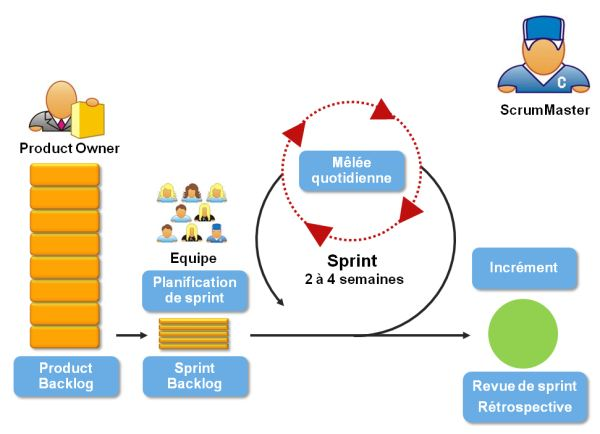
\includegraphics[scale=0.75]{images/scrum}
  \end{center}
  \caption{Schéma décrivant la méthode Scrum}
  \caption*{Source: http://www.agiliste.fr/fiches/guide-demarrage-scrum/}
  \label{scrum}
\end{figure}

\subsection{Scrum avec Open Orchestra}
Au sein du projet Open Orchestra, la méthode Scrum est appliqué. Ainsi des sprint de une semaine avec un daily scrum tous les jours à midi.
De plus, tous les mercredis ou mardi selon les disponibilités une \og cérémonie \fg{} qui comprend la réunion de planification et la rétrospective.
Concernant, la revue de sprint (validation des tâches du sprint) celle-ci n'est pas faite durant une réunion défini mais tout au long du sprint par le product ownver.
 \paragraph{}
 Pour faciliter la mise en place de la méthode Scrum, l'équipe utilise différent outils.
 Tout d'abord Skype et Slack\footnote{Slack est une plateforme de communication réalisée en 2014 qui permet d'intégrer facilement différents outils de service en ligne telle que github, trello, dropbox, google drive, ...)} pour la communication.
  \paragraph{}
 Et enfin Trello pour organiser les tâches, en effet l'équipe posséde un \verb?board? avec différentes colonnes pour organiser les tâches : 
 \begin{itemize}
 \item[]
 \item \textbf{Backlog} : le backlog qui contient les différentes tâches a effectuer pour le projet, les tâches du backlog sont organisées en quatre colonnes (Nice to have, Good, Great, Must have) selon la priorité de la tâche.
 \item[]
 \item \textbf{Support} : Les demandes effectuées par les différentes équipes d'intégrateur d'Open Orchestra au sein d'Interakting.
\item[]
 \item \textbf{Proposition} : Les différentes propositions d'amélioration ou de re-factorisation du code faitent par les membres de l'équipe.
\item[]
 \item \textbf{Bugs} : Les différents bugs rencontrés durant le développement
\item[]
 \item \textbf{Todo} : Les tâches à effectuer durant le sprint en cours.
\item[]
 \item \textbf{Doing} : Les tâches actuellement en développement.
\item[]
 \item \textbf{Blocked} : Les tâches bloquées pour différentes raisons (manque de précision de la tâche, bug empêchant la réalisation de la tâche)
\item[]
 \item \textbf{ToDeploy} : Tâches réalisées qui sont prêtes à être déployé sur le serveur d'intégration.
\item[]
 \item \textbf{ToValidate} : Tâches du sprint en attente de validation par le product owner.
\item[]
 \item \textbf{Failed} : Tâches du sprint non validé par le product owner
\item[]
 \item \textbf{Done} : Tâches du sprint validé par le product owner
 \item[]
 \end{itemize}
Les colonnes \verb?ToDeploy?, \verb?Done? sont uniques a un sprint, il y a donc une colonne \verb?ToDeploy?, \verb?Done? différente pour chaque sprint.
\paragraph{}
Par exemple, une tâche suit un processus, présenté par le schéma~\ref{tache_trello}, bien particulier entre l'intégration de la tâche dans la sprint et sa validation par le product ownver. Ce processus permet de suivre facilement l'avancement ou encore les différents problèmes rencontrés sur les différentes tâches par tous les membres de l'équipe.

\begin{figure}[H]
  \begin{center}
    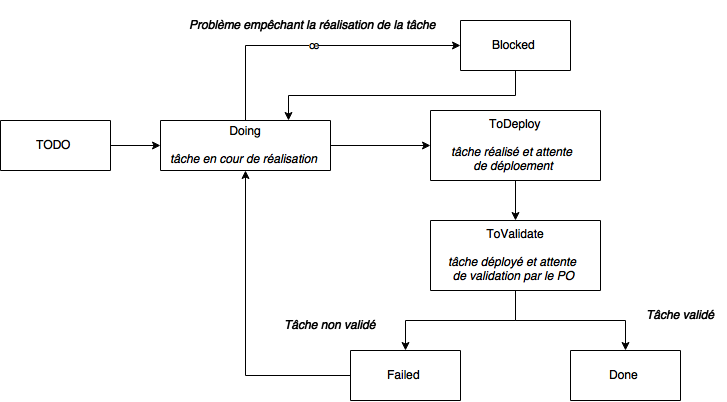
\includegraphics[scale=0.70]{images/tache_trello}
  \end{center}
  \caption{Schéma représentant la progression d'une tâche lors d'un sprint}
  \label{tache_trello}
\end{figure}
\section{Intégration continue}
Pour son développement Open Orchestra utilise les principes de l'intégration continue. 
\newline
\begin{quotation}
L'intégration continue est un ensemble de pratiques utilisées en génie logiciel consistant à vérifier à chaque modification de code source que le résultat des modifications ne produit pas de régression dans l'application développée.
\end{quotation}
\textit{Source wikipedia}

L'utilisation de ces pratiques apporte de nombreux avantages, tout d'abord comme il est indiqué dans la définition cela permet de minimiser les régréssions mais aussi, d'avoir à tout moment un produit (logiciel, site, etc) utilisable.
\paragraph{}
La mise en place de cette technique nécessite différents pré-requis : 
\begin{itemize}
\item[]
\item Dépôt unique de code source versionné
\item Automatisation des tests
\item Un environnement similaire à celui de production
\item Automatiser le déploiement
\end{itemize}

\subsection{Git}
Dans le cadre d'Open Orchestra, le code source est versionné avec git\footnote{Git est un logiciel de versionning décentralisé, c'est-à-dire qu'il n'existe pas un dépôt unique mais un dépôt local pour chaque développeurs.} et utilise GitHub qui est un service web permettant d'héberger un dépôt git. Comme je l'expliquais lors de la présentation d'Open Orchestra, ce dernier est découpé en plusieurs bundles et donc chaque bundle possède son propre dépôt sur GitHub.
\paragraph{}
Open orchestra étant toujours en version bêta, il n'y a pas de realease à proprement parlé. Ainsi le worklow de développement sur github est simplifié car il y a qu'une seule branche stable, la branche master. Les autres branches sont des branches temporaires d'ajout de fonctionnalités ou de correction de bugs. Ce type de workflow est appellé \verb?GitHub flow? et est représenté par le schéma~\ref{github}.
\begin{figure}[H]
  \begin{center}
    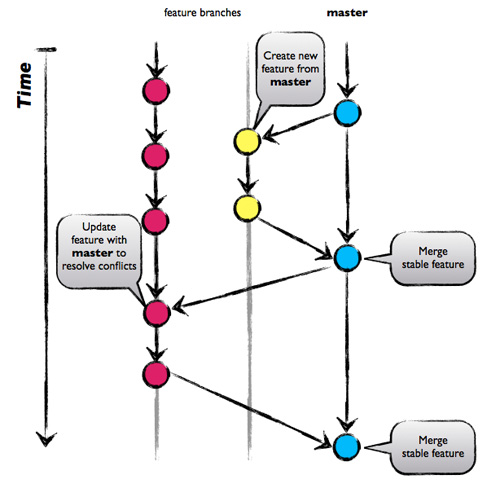
\includegraphics[scale=0.75]{images/github-flow}
  \end{center}
  \caption{GitHub flow}
  \caption*{Source: http://nicoespeon.com/fr/2013/08/quel-git-workflow-pour-mon-projet}
  \label{github}
\end{figure}

\paragraph{}
Ainsi avec ce type de workflow, la modification du code source que ce soit pour corriger un bug ou ajouter une fonctionnalité s'effectue toujours de la même manière : 
\begin{enumerate}
\item[]
\item Mettre à jour sa branche master en local
\item Créer une nouvelle branche en local à partir de master
\item Effectuer les modifications dans cette branche
\item Pousser sa branche sur GitHub (origin)
\item Vérifier que les tests fonctionnnent, je reviendrai plus en détail sur les tests par la suite
\item Ouvrir une pull-request, sur GitHub une pull-request consiste à faire une proposition de modifications, à partir de cette pull-request les différents membres peuvent commenter, valider ou non la modification.
         \item[]
\end{enumerate}

Une fois la pull-request validé, elle peut être mergé avec master, c'est-à-dire inclure la modification dans la branche master.
\paragraph{}
Comme je l'ai précisé en début de section pour le moment Open Orchestra ne posséde pas de branche realease. Toutefois, le projet Open Orchestra est déjà utilisé par des intégrateurs pour réaliser des sites à distanciation de différents clients, ils ne peuvent donc pas utiliser directement la branche master, ils leurs faut des points d'arrêts. 

\paragraph{}
Pour cela, sauf cas particulier (bug bloquant, besoins particulier) la branche master est \verb?taggé? toutes les deux semaines environ ainsi cela permet à l'équipe d'Open Orchestra de continuer le développement  du projet et aux intégrateurs d'avoir une version fixe de la branche master qu'ils peuvent mettre à jour au moment le plus opportun pour eux.  Lorsque Open Orchestra ne sera plus en bêta cela changera la version 1 aura sa propre branche dans laquelle aucune nouveauté sera intégré hormis les corrections de bug.

\subsection{Travis CI}
Lorsqu'une branche est poussée sur l'un des dépôts GitHub du projet, les tests sont automatiquement lancés. Pour cela, les différents dépôts du projet intègrent l'outil \verb?Travis CI?. Travais CI est un service qui est lié a GitHub, il permet de déclencher un certain nombre de tâches lors d'événements sur le dépôt. Dans le cas d'Open Orchestra Travis CI permet de lancer les tests unitaires après chaque \verb?push? sur un dépôt. Un des avantages de travis est qu'il se configure très facilement grâce un fichier yaml.
\paragraph{}
Par exemple le fichier de configuration travis d'un des dépôts d'Open Orchestra 
\begin{verbatim}
    language: php

    php:
          - 5.4

    install:
          - composer install --prefer-dist --no-progress
 
    script: ./bin/phpunit
\end{verbatim}

Indique que le langage utilisé est php et que les tests doivent être exécutés avec la version 5.4 de php et enfin avant d'exécuter \verb?phpunit? pour lancer les tests il est demandé a travis de faire un \verb?composer install? pour récupérer les dépendances du projet. Ensuite, à partir de ce fichier de configuration Travis CI est capable de créer l'environnement pour effectuer les tests, il est bien sûr possible d'aller plus loin dans la personnalisation de l'environnement en allant cherchant d'autres dépendances avec \verb?apt-get install? par exemple ou encore de demander à être notifié par email si les tests ne passent pas.

\subsection{Déploiement}
Le déploiement sur un serveur de production n'est pas toujours une tâche facile (uploader le code, mettre à jour les dépendances, lancer les migrations de la base de données, vider le cache, etc)  or pour permettre une intégration continue il est nécessaire de déployer régulièrement son application, il semble donc nécessaire d'automatiser cette tâche, pour cela il existe de nombreux outils. 
\paragraph{}
En ce qui concerne Open Orchestra nous utilisons \verb?Capistrano?. \verb?Capistrano? est un outil écrit en Ruby qui permet d'exécuter des scripts sur un ou plusieurs serveurs. Il est principalement utilisé pour faire du déploiement, mais il permet aussi de créer ses propres tâches, par exemple pour Open Orchestra nous l'utilisons aussi pour lancer des tests de charge, avec Jmeter, directement sur le serveur d'intégration.
\paragraph{}
Un autre avantage de \verb?Capistrano? est qu'il permet de revenir facilement sur une version précédente de votre application grâce à une architecture de dossier que met en place \verb?Capistrano? dans le dossier de votre application sur serveur : 
\begin{verbatim}
/app/
       releases/ Contient un dossier pour chaque déploiement estampillé
       current   Lien symbolique pointant vers un dossier de release spécifique
       shared/   Contient les données partagées entre chaque déploiement
\end{verbatim}
Ainsi, si un déploiement provoque des erreurs, il suffit de faire pointer le lien symbolique \verb?current? vers une autre version.

\section{Qualité}
L'équipe d'Open Orchestra essaye de fournir un produit de qualité que ce soit au niveau du code, du couplage ou encore du fonctionnel. Pour cela différentes pratiques, outils sont mises en place.
\subsection{Qualité du code}
Tout d'abord au niveau du code Open Orchestra utilise le standard PSR-2. PSR-2 est un ensemble de recommandations sur le style et l'organisation du code dont voici les plus importantes : 
\begin{itemize}
\item[]
\item La tag de fermeture \verb?\?>. doit être omis de tous les fichiers contenant uniquement du PHP
\item Tous les fichiers PHP doivent se terminer par une ligne vide.
\item La visibilité doit être déclarée sur toutes les propriétés et méthodes.
\item L'ouverture des accolades pour les classes, les méthodes doivent figurer sur la ligne suivante, les accolades de fermeture doivent figurer sur la ligne suivante après le corps de la classe.
\item Il doit y avoir un espace après la structure clé de contrôle et pas d'espace après la parenthèse ouvrante et avant la parenthèse fermante
\item Il doit y avoir un espace entre la parenthèse fermante d'une structure de contrôle et de l'accolade
 ouvrante
 \item L'accolade fermante d'une structure de contrôle doit être sur la ligne suivante après le corps
 \item[]
\end{itemize}
\paragraph{}
Utiliser cette recommandation permet une harmonisation du code et ainsi il est plus simple pour toute l'équipe de relire et reprendre le code d'un autre membre, mais aussi pour tous les développeurs qui utilisent Symfony 2 puisque ce dernier utilise aussi les recommandations PSR-2
\paragraph{}
Lors de revue de code des pull-request, il n'est pas toujours aisé de détecter l'utilisation des bonnes pratiques ou non. Il existe des outils qui permettent d'analyser le code automatiquement et de détecter les oublie lors de la revue.
\paragraph{}
Pour le projet Open Orchestra deux outils sont utilisés : 
\paragraph{}
Tous d'abord, Code Climate s'interface avec les dépôts c'est-à-dire que lors d'un push le code est analysé.

Code Climate permet de détecter la duplication de code, la couverture des tests, la qualité globale du projet. De plus, il fournit une note qui indique la qualité globale du dépôt. 
Le second outil est SensioInsignt qui fonctionne de la même façon que Code Climate mais en supplément des vérifications sur les bonnes pratiques de Symfony 2.
\subsection{Test}
Le plus grand intérêt des tests sont qu'ils permettent de réduire les régressions lorsque l'on applique des modifications à une application. En effet, lorsqu'une application devient assez conséquente il n'est pas toujours aisé d'anticiper toutes les répercutions lorsque l'on modifie une portion de code. Les tests permettent donc de tester l'ensemble de l'application et ainsi vérifier que cette dernière fonctionne toujours correctement après les modifications effectuées. 
De plus, ils sont en général gage de qualité
 \paragraph{}
 Il existe deux grandes familles de test, Tous d'abord les tests unitaires qui permettent de vérifier que chaque méthode et fonction fonctionne correctement, les tests doivent être indépendant au maximum les uns des autres pour cela il existe les mocks qui sont des objets qui permettent de simuler le comportement d'objets \og{}réels\fg{}.
 D'autre part les tests fonctionnels qui eux contrairement aux tests unitaires vérifies les fonctionnalités de bout en bout. c'est-à-dire que du routing jusqu'au vue en passant par le modèle et le controlleur.
  \paragraph{}
 Avec Symfony, il est assez facile de créer des tests puisqu'il intègre la bibliothèque PHPUnit qui fournit un framework de test complet, de plus pour les tests fonctionnels Symfony propose une classe WebTestCase qui permet d'initier le noyau de Symfony, cette classe fournit notamment un objet \verb?client? qui permet d'effectuer des requêtes HTTP sur son application et un crawler pour vérifier le résultat retourné par la requête.
  \paragraph{}
  En plus des différents tests au niveau du code serveur, Open Orchestra possède aussi des tests de charges réalisés avec Jmeter. Jmeter est un logiciel qui permet de tester les performances d'une application en simulant des utilisateurs. Concrètement pour effectuer un test, il suffit décrire un scénario fonctionnel c'est-à-dire un enchainement d'action (visiter une url, remplir un formulaire, etc) que Jmeter devra effectuer lors du test et un nombre d'utilisateur qui réaliseront ce scénario.
  
  \paragraph{}
  Lorsque que Jmeter effectue un test, il fournit un tableau de résultat avec différentes données telles que le temps de réponse d'une url, le pourcentage d'erreur, etc) ainsi cela permet de voir comment réagissent les différentes fonctionnalités de son application avec un nombre important d'utilisateur.
\subsection{Qualité fonctionnel}
Un point important d'une application est son ergonomie, concernant le projet Open Orchestra des consultants fonctionnels ont émit différentes propositions afin d'améliorer l'ergonomie. Les différentes propositions sont recueillies au sein d'un board Trello prévu à cet effet avec différentes colonnes (Propositions, Propositions validés par un expert fonctionnel, Propositions acceptées par Open Orchestra). 
  \paragraph{}
  Ainsi lorsqu'une proposition est validée par un expert fonctionnel, nous en parlons en cérémonie pour savoir si elle doit être ou non intégrée au backlog du projet. 